\section{Capital Asset Pricing Model (CAPM)}
\label{sec:capital_asset_pricing_model}

\subsection{Intuition of the CAPM \texorpdfstring{$\beta$}{beta}}
\begin{equation}
    \label{eq:capm}
    E[R_i] = R_f + \beta_i (E[R_m] - R_f)
\end{equation}

The Capital Asset Pricing Model is a model that describes the expected returns of an asset as a function of its exposure to systematic risk.
The model is given by Equation \ref{eq:capm}, where:
\begin{itemize}
    \item $E[R_i]$ is the expected return of asset $i$
    \item $R_f$ is the risk-free rate
    \item $\beta_i$ is the asset's beta
    \item $E[R_m]$ is the expected return of the market
\end{itemize}

Notice that according to the model, a firm's expected return is only a function of its exposure to the market's risk.
This comes from a fundamental belief that in the long-run, any firm-specific/idiosyncratic risk can be diversified away, therefore
investors look to be compensated for the risk that cannot be diversified away, which is the market risk.

To estimate the CAPM beta for firms, we regress a firm's historical returns against the market's returns, and take the slope of the line of best fit.
This is given by Equation \ref{eq:beta_regression}:
\begin{equation}
    \label{eq:beta_regression}
    R_i - R_f = \alpha + \beta_i (R_m - R_f) + \epsilon
\end{equation}

Where:
\begin{itemize}
    \item $R_i$ is the firm's return
    \item $R_f$ is the risk-free rate
    \item $R_m$ is the market return
    \item $\alpha$ is the intercept of the regression line
    \item $\beta_i$ is the slope of the regression line
    \item $\epsilon$ is the error term
\end{itemize}

$\alpha$ is also known as Jensen's alpha, it is a reflection of how much a firm under or outperforms the market, given its beta.
In a world where CAPM perfectly models a firm's returns, $\alpha$ should be zero.

\begin{table}
    \centering
    \begin{tabular}{|c|c|c|}
        \hline
        \textbf{Asset} & \textbf{Beta}\\
        \hline
        AAPL & 1.10\\
        GE & 0.92\\
        IBM & 0.75\\
        KO & 0.49\\
        MSFT & 1.14\\
        \hline
    \end{tabular}
    \caption{Sample assets and their CAPM betas}
    \label{tab:sample_assets_capm}
\end{table}

Table \ref{tab:sample_assets_capm} shows the CAPM betas for a few sample assets. Higher beta assets are 'riskier' since they are more 
exposed to the market's risk, and therefore should have higher expected returns.

We can see this more clearly in figure \ref{fig:historical_expected_returns_vs_beta}, where we plot the historical 
average annualized return against a firm's beta. We can see that there is a positive relationship between beta and expected return.
In this same plot we add the Security Market Line (SML), which is the line that represents the expected return of an asset given its beta.
We notice that not all stocks lie on this line, stocks above this line are out performing their expected return, and stocks below this line are under performing their expected return.
But, this evaluation of performance is only valid if we assume that the CAPM is a perfect model of the market, which it may not be.
To note is that we already discussed the Fama-French 3 factor model which is already an extension showing that the CAPM model is underspecified.

\begin{figure}
    \centering
    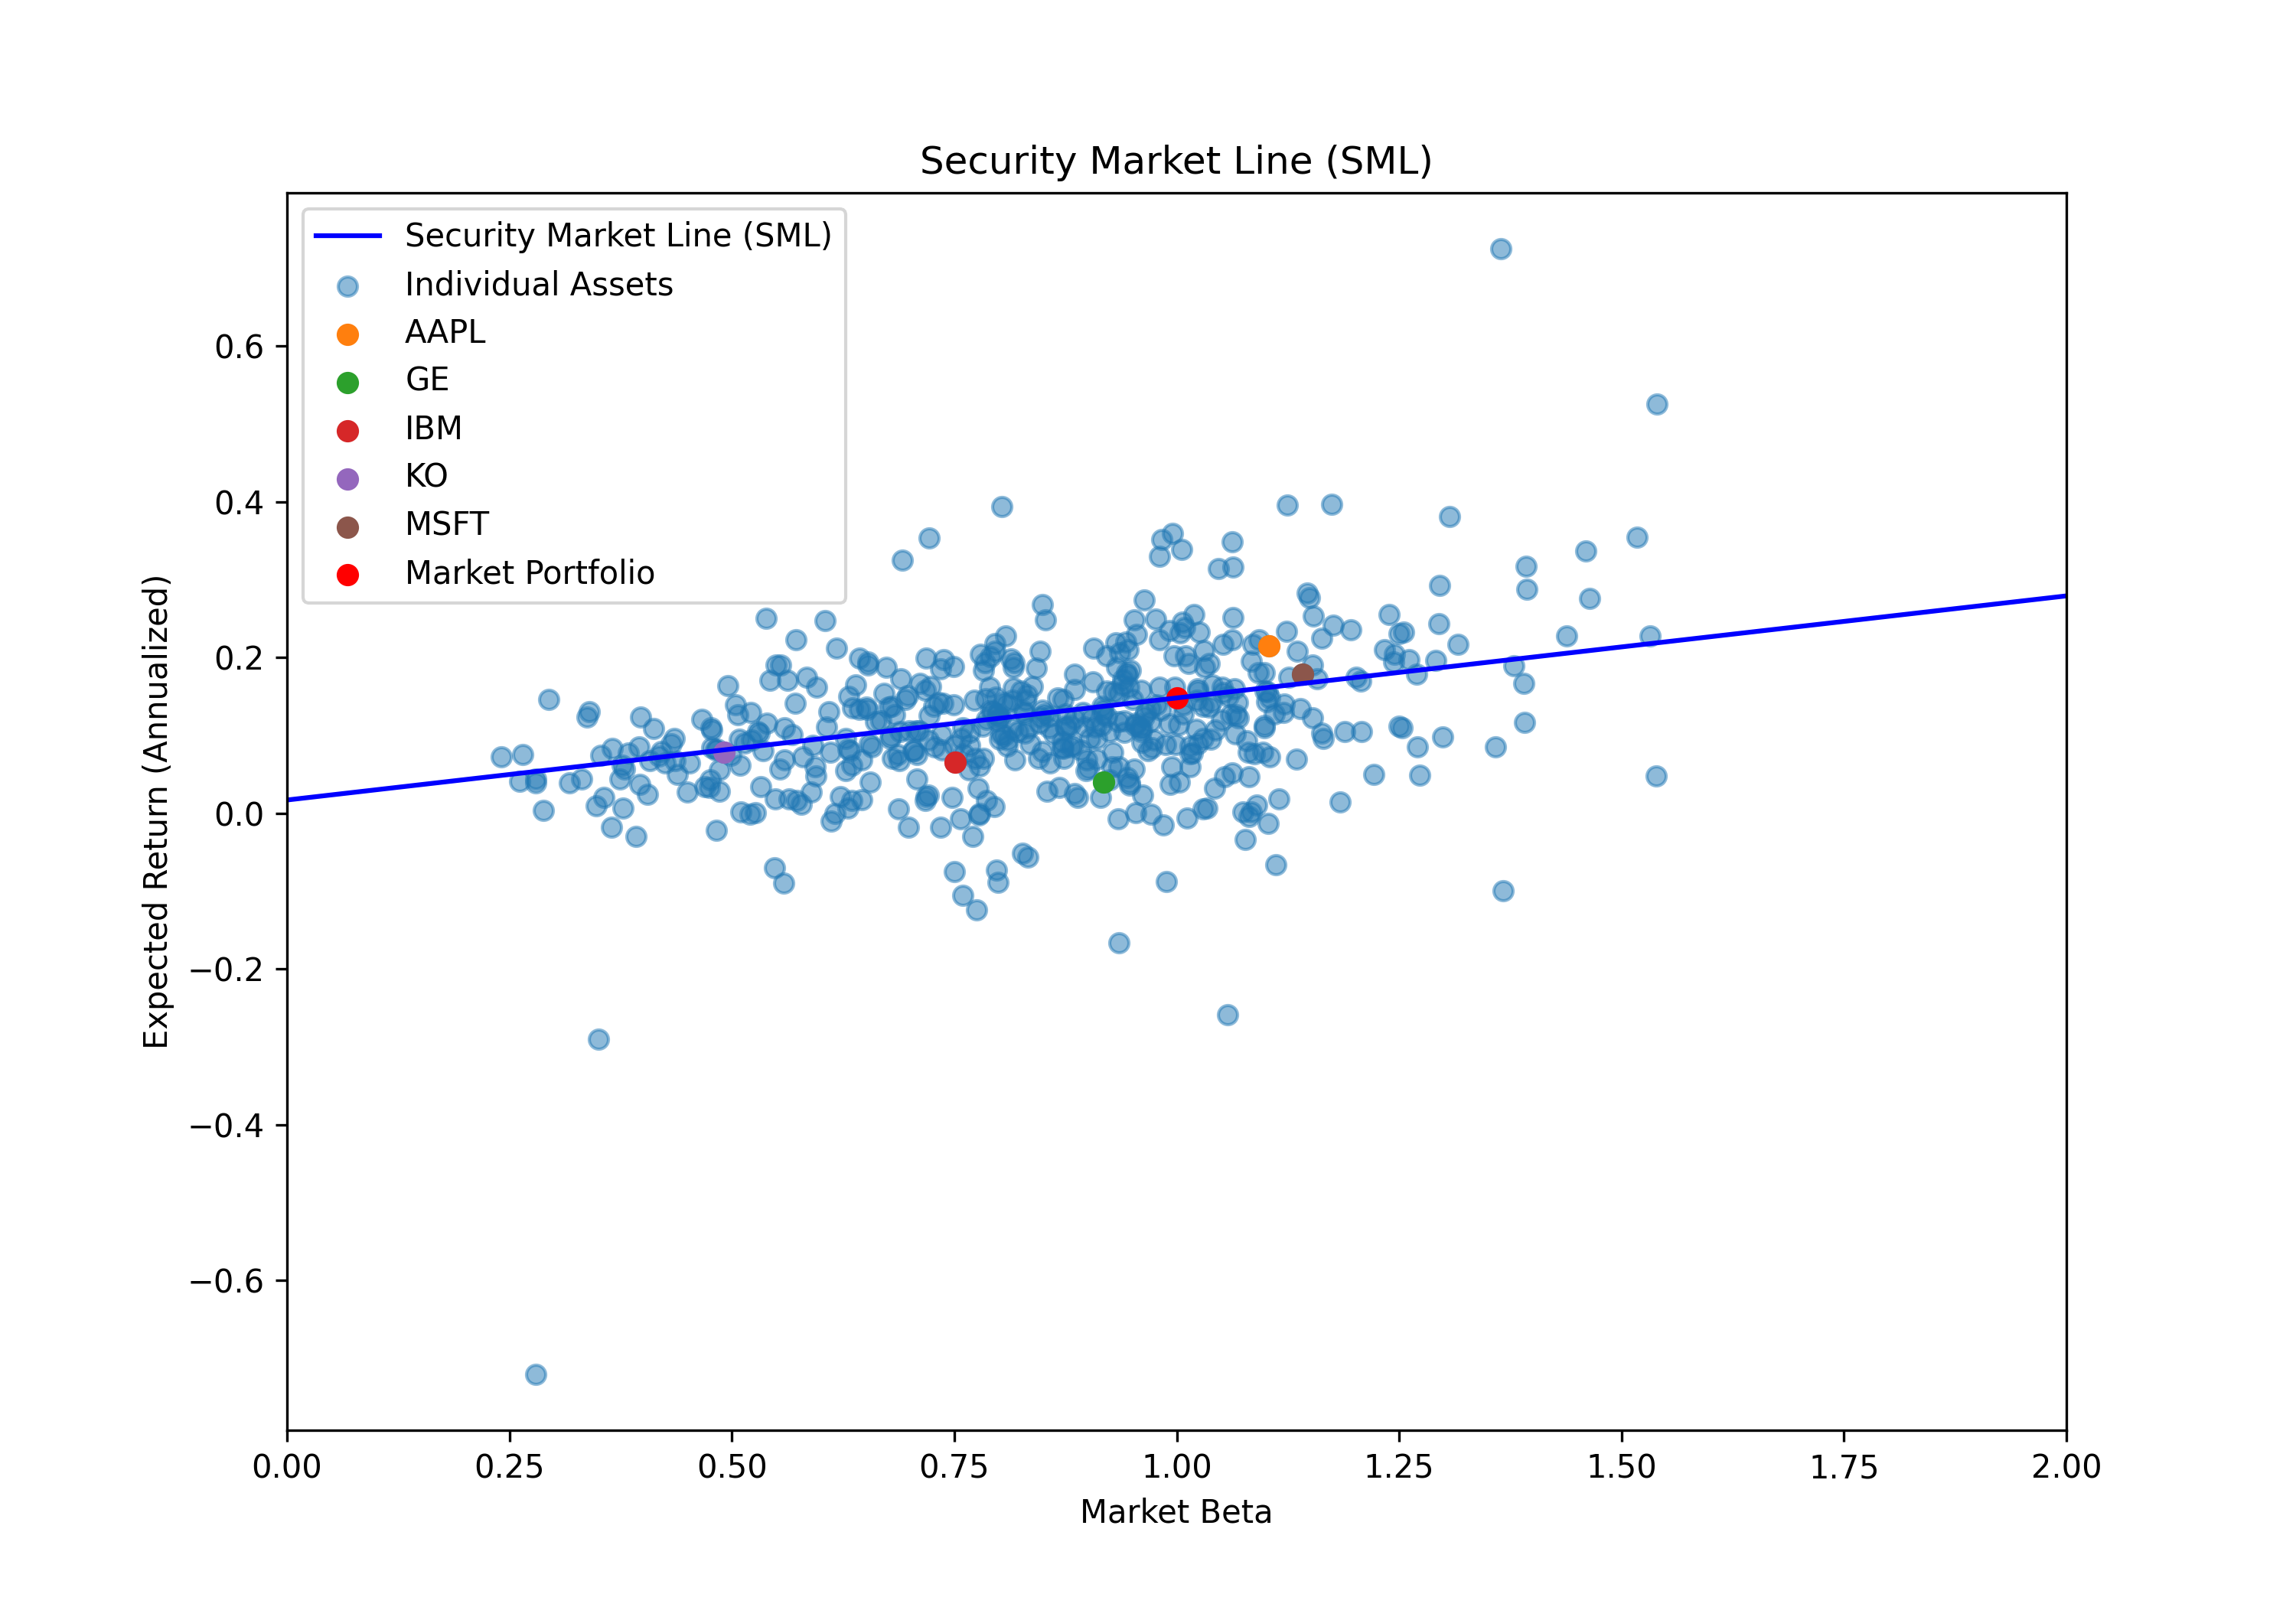
\includegraphics[width=0.8\textwidth]{../figs/historical_expected_returns_vs_beta.png}
    \caption{Plot showing the historical average annualized return against a firm's beta}
    \label{fig:historical_expected_returns_vs_beta}
\end{figure}

Working backwards, we can get the CAPM expected return for a firm by multiplying each firm's CAPM beta by the average market return over the period.
Table~\ref{tab:sample_asset_capm_and_expected_return_table} shows the expected returns for a few sample assets, given their CAPM and the average market return.

\begin{table}
    \centering
    \vspace{1em}
    \begin{tabular}{lrrr}
\toprule
symbol & capm\_beta & capm\_expected\_return & std\_dev\_ann \\
\midrule
AAPL & 1.10 & 0.16 & 0.25 \\
GE & 0.92 & 0.14 & 0.29 \\
IBM & 0.75 & 0.12 & 0.21 \\
KO & 0.49 & 0.08 & 0.16 \\
MSFT & 1.14 & 0.17 & 0.24 \\
\bottomrule
\end{tabular}

    \caption{Sample assets and their expected returns using the CAPM}
    \label{tab:sample_asset_capm_and_expected_return_table}
    \vspace{1em}
    \centering
\end{table}

\subsection{Cost of Capital - DDM vs CAPM}
% Explain the cost of capital
% Explain how to calculate it using the DDM
% Explain how to calculate it using the CAPM
% Explain the fundamental intuition of the difference between the two

Recall the definition of cost of capital, and that it is synonymous with expected return.
We previously explored using the Dividend Discount Model (DDM) to estimate the cost of capital. The intuition of the 
DDM is that a stock price represents the present value of all future cashflows, where we proxy all future cashflows using a dividend and expected growth rate.
A DDM feels more realistic the better we can forecast a firm's future dividends, as well as their dividend growth rate, given that they pay dividends.
If we start to consider that there are firms that don't pay dividends at all, or that the dividend growth rate is hard to forecast, we start to see the limitations of the DDM.
Additionally, if we are investors that don't care about dividend payouts, we may not find the DDM useful at all.

The CAPM, on the other hand, is a model that is based on the idea that investors are compensated for the systematic risk they take on. If a risk can be diversified away, then
investors shouldn't be compensated for it (as they can get rid of it).
If markets are efficient, and investors are rational, then the current stock price should reflect all available information about a firm.
There is no need to forecast dividends, or growth rates, or anything else about the firm. We only need to know the firm's exposure to systematic risk.
